% ==========================================================================================
% 
%                                     RV EXTRACTIONS
% 
% ==========================================================================================
\newpage
\section{Additional details}\label{appendix:RV_extraction}

\begin{SCfigure}[1][!ht]%
    \begin{wide}  
    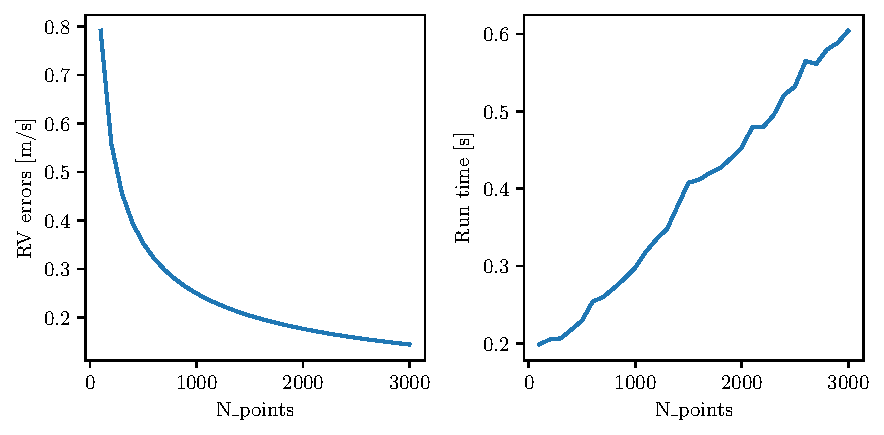
\includegraphics[scale=0.72]{figures/err_vs_run_time.pdf}
    \caption{Resulting error in extracted radial velocity shift between two observations (left) and run time of that computation (right) as a function of number of sampled points in the interpolation.}
    \label{fig:err_vs_run_time}
\end{wide}
\end{SCfigure}

\begin{SCfigure}[1][!ht]%
    \begin{wide}  
    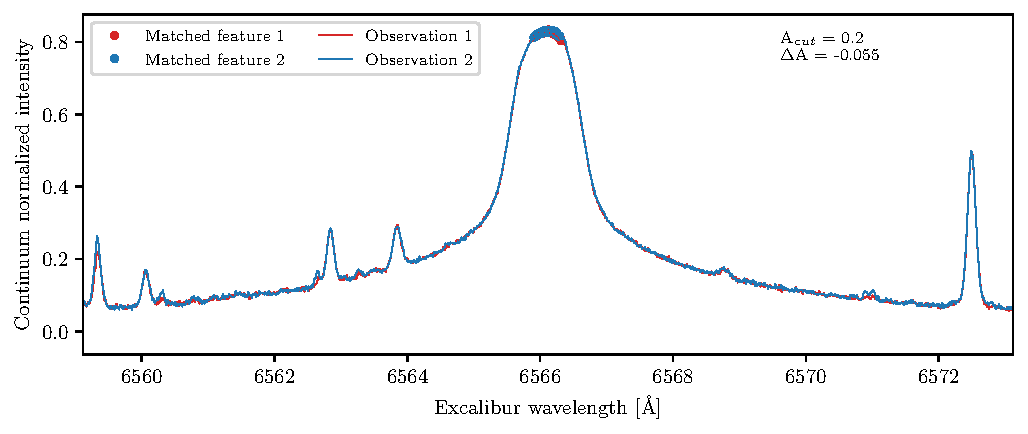
\includegraphics[scale=0.72]{figures/bad_match_example.pdf}
    \caption{Example of a bad match that made it through the filters. This match is actually correct, but yields a bad result because it is too broad for the standard data slice size.}
    \label{fig:bad_match_example}
\end{wide}
\end{SCfigure}

\subsection*{Computational run times}
For running the analysis I have used a Macbook M1 pro (2021).

\subsubsection*{Calibration}
\begin{itemize}
    \item Fitting super-Gaussian to 17,068 LFC lines takes about 45 seconds (one core).
    \item Computing the interpolation function and fitting the polynomials takes less than a second.
\end{itemize}

\subsubsection*{RV extractions}
\begin{itemize}
    \item Finding all features in 188 files takes just about 1 minute (one core).
    \item The run time for computing the $\Delta V_r^{ij}$ matrix of course scales as $N^2$. The following times are for running the computation in parallel on 6 CPU cores:
    \begin{itemize}
        \item[] \begin{tabbing}
            HD 34411 \hspace{0.5 cm} \= $N_{\text{files}} =$ 188 \hspace{0.5 cm} \= $N_{\text{features}} =$ 12,608,511 \hspace{0.25 cm} \= :\qquad 121 minutes \\

            HD 10700    \> $N_{\text{files}} =$ 174 \> $N_{\text{features}} =$ 9,008,471   \> :\qquad 91 minutes \\
            HD 26965    \> $N_{\text{files}} =$ 114 \> $N_{\text{features}} =$ 5,777,355   \> :\qquad 62 minutes \\
            HD 101501   \> $N_{\text{files}} =$ 45 \> $N_{\text{features}} =$ 815,719     \> :\qquad 9 minutes \\
        \end{tabbing}
    \end{itemize}
    \item The subsequent reduction of the $\Delta V_r^{ij}$ matrix takes up to five minutes on one core.
\end{itemize}

% ==========================================================================================
% 
%                                     RESULTS
% 
% ==========================================================================================
\newpage
\section{Additional results}\label{appendix:results}

\small{Relative radial velocities computed for three more stars: HD 101501, HD 10700, and HD 26965. In each figure the top shows my final extracted RV shifts using excalibur calibrated, barycentric-corrected data (data column \texttt{bary\char`_excalibur}), the center shows Zhao et al.'s results using a chunk-by-chunk (CBC) analysis technique \cite{yale_data}, and the bottom shows residuals from subtracting Zhao's results from mine. }

\begin{SCfigure}[1][!ht]%
    \begin{wide}  
    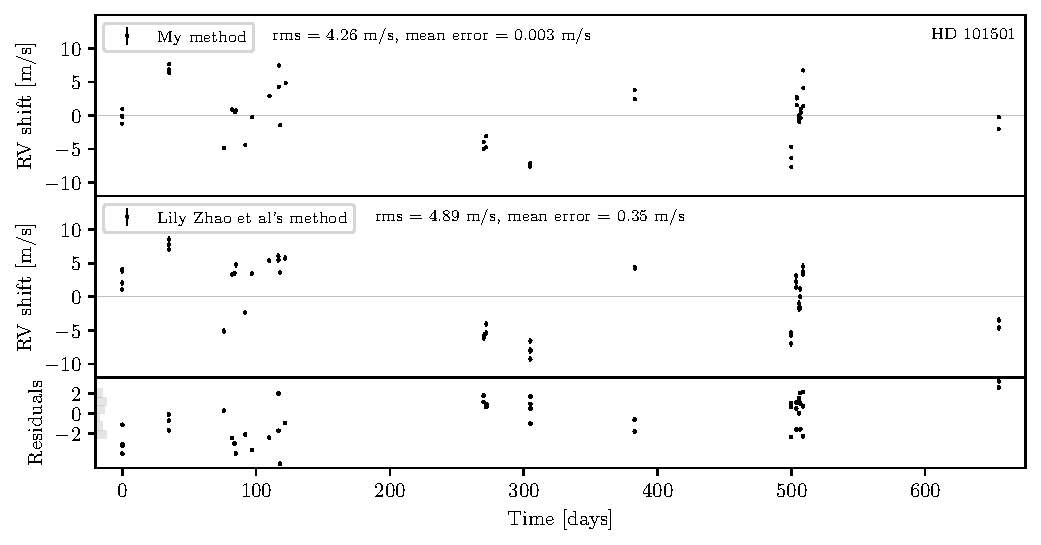
\includegraphics[width=\textwidth]{figures/HD101501_barycentric_rv_vs_lily.pdf}
    \caption{HD 101501\newline 45 observations made between 2019-2-10 and 2020-11-26.}
    \label{fig:HD101501_rvs}
\end{wide}
\end{SCfigure}

\vspace{-0.75cm}

\begin{SCfigure}[1][!ht]%
    \begin{wide}  
    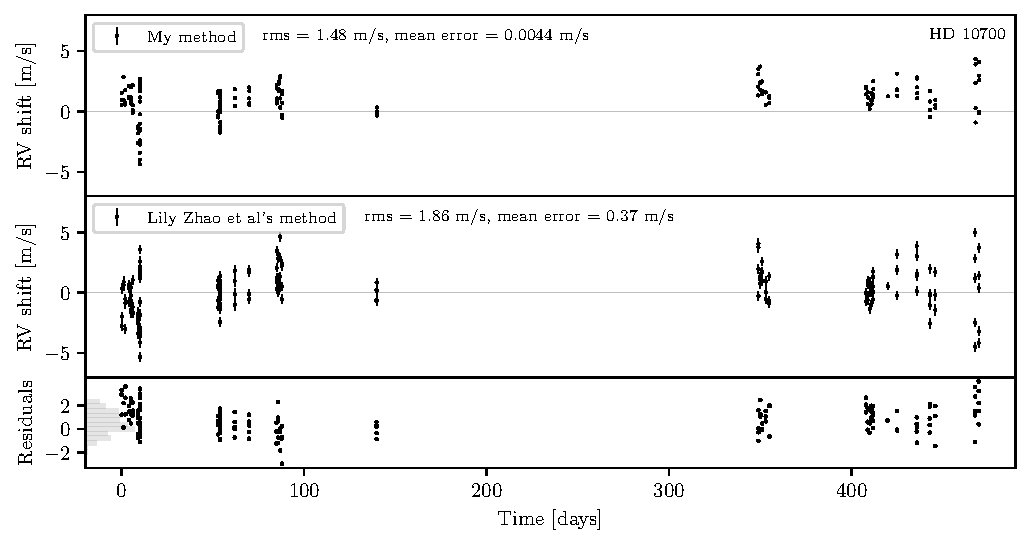
\includegraphics[width=\textwidth]{figures/HD10700_barycentric_rv_vs_lily.pdf}
    \caption{HD 10700\newline 174 observations made between 2019-8-15 and 2020-11-27.}
    \label{fig:HD10700_rvs}
\end{wide}
\end{SCfigure}

\vspace{-0.75cm}

\begin{SCfigure}[1][!ht]%
    \begin{wide}  
    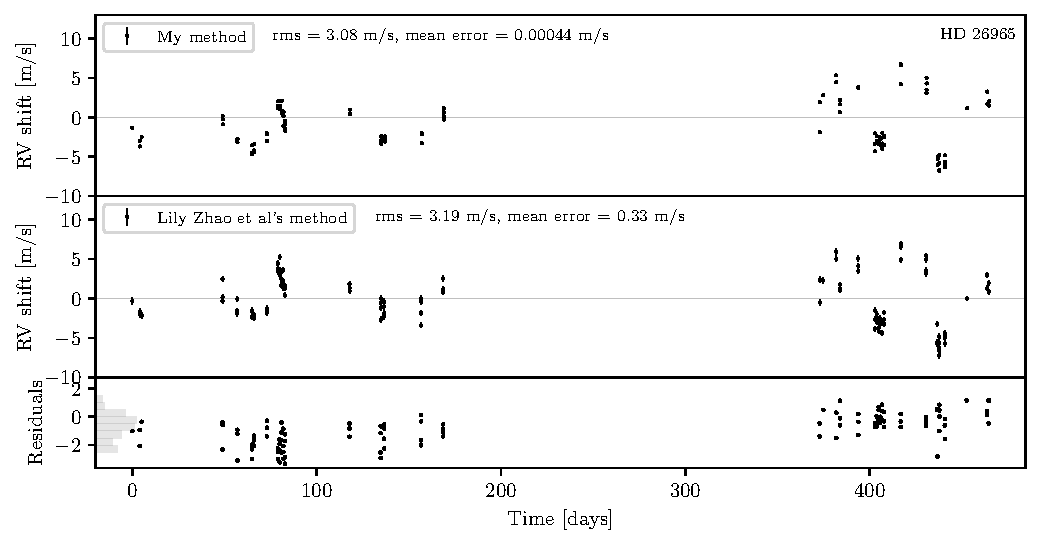
\includegraphics[width=\textwidth]{figures/HD26965_barycentric_rv_vs_lily.pdf}
    \caption{HD 26965\newline 114 observations made between 2019-8-20 and 2020-11-27.}
    \label{fig:HD26965_rvs}
\end{wide}
\end{SCfigure}
